\chapter{Algorithm and Model Creation}

\section{Original Invitation Election Algorithm Overview}

A state machine for the election portion of the invitation-election algorithm is shown in Figure \ref{fig:statemachine}.
In the normal state, the election algorithm regularly searches for other coordinators to join.
When another coordinator is identified, the identifying coordinator will attempt to invite the other coordinator to their group.
In the invitation election algorithm, processes are assigned a priority based on their process ID.
The coordinator with the highest priority is the first to send invites.
After a brief delay, if it appears that coordinator did not send their invites, the next highest process will send their invites.
If a coordinator accepts an invitation, it will forward the invite to its group members.
Processes that receive an invite that are not already in an election will accept the invite.
Once a timeout expires, the coordinator will send a ``ready'' message with a list of peers to all processes that accepted the invite.
The invited processes have timeouts for when they expect the ready message to arrive.
If the message does not arrive in time, the process will enter the recovery state where it resets to a group with itself as the only member.

\begin{figure*}[!t]
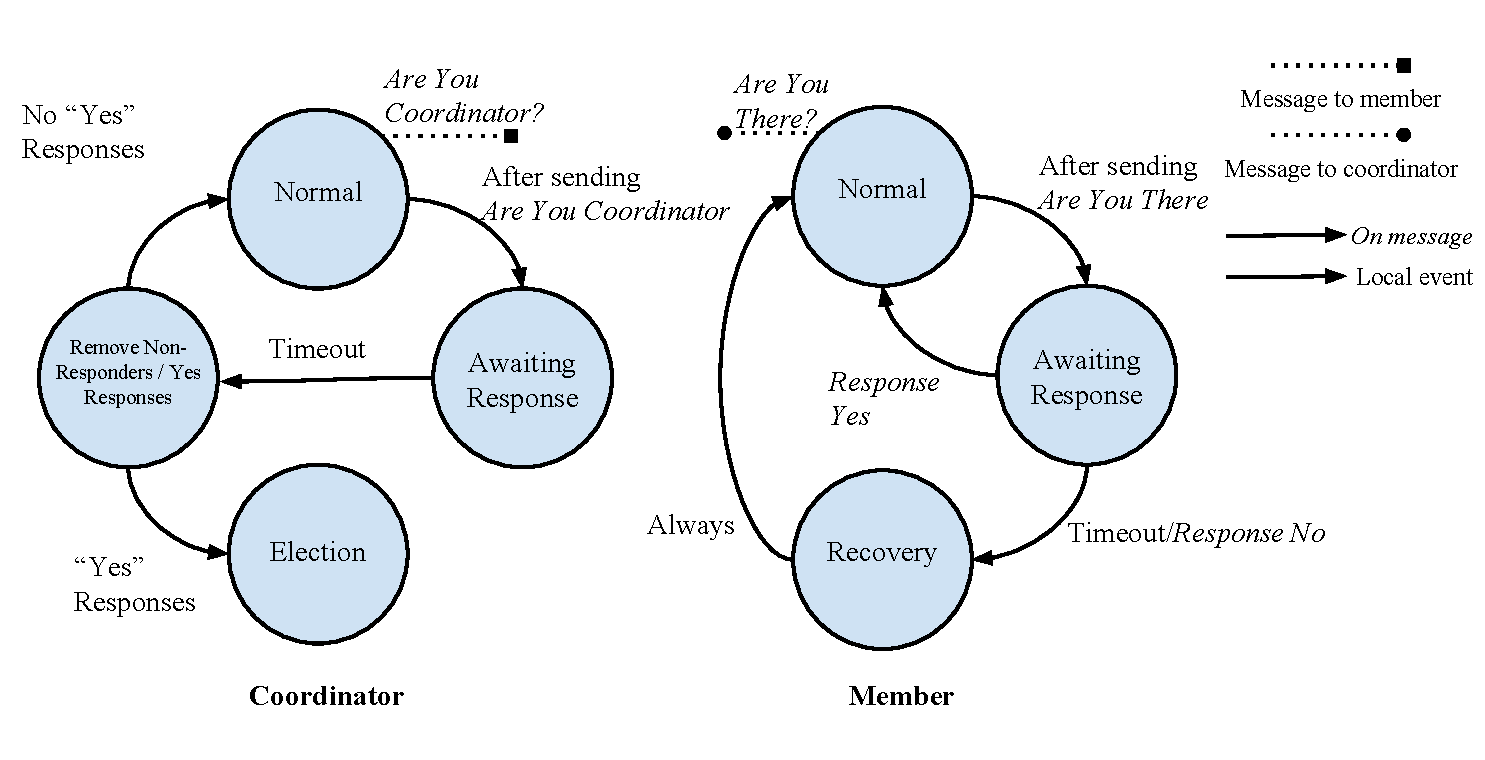
\includegraphics[width=\linewidth]{MaintainStateDiagram.pdf}
\caption[State machine for maintaining a group]{State machine for maintaining a group. The \ac{AYC} messages are the same as those in Figure \ref{fig:statemachine}. \ac{AYC} and \ac{AYT} are periodically sent by processes, and responses to those messages are immediately sent by the receiving process. In the modified algorithm, the member does not enter the recovery state if they do not receive an AYT response before the timeout expires.}
\label{fig:statemachine2}
\end{figure*}

Once a group is formed it must be maintained.
To do this, processes occasionally exchange messages to verify the other is still reachable.
The interaction is shown in Figure \ref{fig:statemachine2}.
Coordinators send ``Are You Coordinator'' messages to members of its group to check if the process has left the group.
Group members send ``Are You There'' messages to the coordinator to verify they haven't been removed from the group and to ensure the coordinator is still alive.
If processes fail to reply to a received message before a timeout, they will leave the group.
Leaving the group can initiated by the coordinator removing the process, or the process can enter a recovery state and leave the group, forming a new group with itself as the only member.

\section{Execution Environment}

Execution occurred in a real-time, partially synchronous environment.
The execution environment was subject to omission failures.
Processes synchronized their clocks and executed steps of the election algorithm at predefined intervals.
Processes with clocks that were not sufficiently synchronized could not form groups.
For this work, process execution occurred in an environment where the clocks were sufficiently synchronized to consistently form groups.
In the real-time environment, messages that were delayed and missed their real-time deadlines had the same appearance as an omitted message.
The execution environment for the election algorithm had an omission fault occurrence modeled as a Bernoulli trial.
In this model, each message had some probability $p$ of being delivered within the timing constraints imposed by the real-time schedule.
For the purpose of analyzing the effects of omission failures, processes were not subject to other faults.

\section{Model Construction}

A process can construct a Markov chain if its observations are consistent with the transition probabilities the process can determine with its observable state.
In each election, a process has some probability of joining a given process' group.
Let $\Pr(i \rightarrow j)$, be the probability the outcome of an election is $i$ being a member of $j$'s group.
Since every process must be a member of some group:

\begin{equation}
\sum^{j} \Pr(i \rightarrow j) = 1.
\label{eq:prob-consistent-1}
\end{equation}

Let $\Pr(i \rightarrow j | i \in k)$ be the probability $i$ joins $j$ at the end of an election given $i$ starts in $k$'s group at the start of the election.
A similar relationship to Equation \ref{eq:prob-consistent-1} must exist for this circumstance:

\begin{equation}
\sum^{j} \Pr(i \rightarrow j | i \in k) = 1.
\label{eq:prob-consistent-2}
\end{equation}

A leader process $j$ can construct a Markov chain iff, for every $i$ that can join $j$'s group:
\begin{equation}
\Pr(i \rightarrow j | i \in k) = \Pr(i \rightarrow j), i \neq j \neq k
\label{eq:mod-req-a}
\end{equation}
where $i \in k$ is a state where $i$ is in $k$'s group.
Therefore, the probability of $i$ joining $j$'s group must be independent of $i$'s membership at the start of the election.
Equation \ref{eq:mod-req-a} enforces the probability $j$ observes some process $i$ joining its group is independent of $i$'s previous membership, which is hidden to $j$ unless $i$ was in $j$'s group.
From Equations \ref{eq:prob-consistent-1} and \ref{eq:prob-consistent-2}:

\begin{equation}
\sum_{n \neq j} \Pr(i \rightarrow n | i \in k) = \sum_{n\neq j} \Pr(i \rightarrow n).
\label{eq:mod-req-b}
\end{equation}

If more than one process can create a Markov chain, an algorithm which allows for that circumstance will have undesirable behavior.
Suppose there are three processes A, B, and C.
Without loss of generality, assume C is in A's group.
For B to be able to construct a Markov chain, it must be equally likely that C leaves A's group to join B's as it is likely C would join B given it was not in A's group.
In a system with no omission faults, ideally, a process will join a group and never leave it, especially if the election algorithm is being used to find a consensus value.
Therefore, we restrict model construction to the highest priority process.

\section{Modified Election Algorithm}

The complete, modified election algorithm is listed in the appendix.

\subsection{State Determination}

% Show that the state of the group in the ready set of the orignal algorithm is an N set.
% Show that the members also have an N set.
In the Garcia-Molina version of the algorithm, processes distribute a list of processes that have accepted their invite.
Let $i$ be the coordinator of a group distributing ready messages.
The process $i$ has a list of processes who have accepted its invite.
Let $\varphi_x$ be a wff indicating some process $x$ is part of $i$'s group.
Let $G = \{ \varphi_x | x \in AcceptedInvite \} \cup \{ \varphi_i \}$ be the set of processes that have accepted $i$'s invite.
To finalize the group, $i$ will distribute $G$ to each process described in $G$.
If a processes does not receive $G$ it will not be in the group.

\begin{thm}
    In the original algorithm, each process is MSDND secure on $\varphi_x$ for each $x$ that is not $i$ or itself ($j$).
\end{thm}

\begin{proof}
\begin{case}
    The case where $x = i$ or $x = j$.
\end{case}

If we assume the authenticity of messages is not questioned in this environment, a ready message from $i$ must mean $i$ is a part of the group.
Therefore, $i$'s inclusion in the group is MSDND insecure to $j$.

If $j$ accepts the ready message, that process will be a part of the group in $G$ and since $j$ knows its own state, $j$ knows it is a part of $G$.

\begin{case}
    The case where $x \neq i$ and $x \neq j$.
\end{case}

For process $i$, $i$ distributes $G$ to each other process in $G$.
Let $Q$ be some set of processes that do not receive the $G$ set.

\begin{table}[h!]
\centering
\small
\begin{tabularx}{\linewidth}{l X X}
1. & $I_{j,i} G \forall j \in G $ & $i$ distributes the list of processes that have accepted the invite.  \\
2. & $\neg(B_x I_{x,i} G \wedge T_{x,i} G) \forall x \in Q$ & Processes in $Q$ do not receive $G$. \\
3. & $B_x I_{x,i} G \wedge T_{x,i} G \forall x \not \in Q$ & Processes not in $Q$ receive $G$. \\
    4. & $w \not \vDash V_{B_x G}^{j}(w) \forall \{x | x \not \in \{i,j\}\}$ & $j$ does not know which processes received $G$ \\
\end{tabularx} \\~\\
Therefore, the receipt of $G$ by other members of the group is MSDND secure to $j$.
\label{tab:readynsetproof}
\end{table}
\end{proof}

\begin{cor}
    The set of processes in the ready message is an $N_i$ set, where $i$ the group's coordinator.
\end{cor}

Because every wff in $G$ is MSDND secure, $G$ must be an $N_i$ set, and $L_i = \emptyset$.
As a consequence, the group leader only has an estimate of the system, which may be an overestimate ($M_i \subseteq N_i$).

% Show that with the ready ack, the leader has an L set.
With a ready acknowledgment message from members of the group, the leader can construct an $L_i$ set, which underestimates the state of the system.
From the previous chapter, we have shown that with message passing and omission, at least one process is left insecure to the other.

\begin{thm}
    If a process $j$ sends a ready acknowledgment message to $i$, $j$'s inclusion in the $i$'s view of the system state is MSDND secure to $j$.
\end{thm}

\begin{proof}
When $j$ sends the ready acknowledgment message to $i$, it is uncertain if the acknowledgment message is actually delivered.
From Theorem \ref{case:generalsn0}, we know that $j$ is now MSDND insecure to $i$, but $i$ is secure to $j$.
Using the ready acknowledgment messages, $i$ can then valuate $B_i B_j \varphi_j$ for every $j$ sending an acknowledgment message.
\end{proof}

Once the ready acknowledgment messages have been sent to the leader, the group can begin to interact.
As it is impossible for the members of the group to be distributed the $L_i$ set, they must operate using the $N_i$ set they received from the coordinator.
Messages from other processes which could only have been sent if they are a part of the $M_i$ set can leak to the receiving processes their receipt of the $G$ set from $i$.
For the purpose of model construction, the determination of members of $M_i$ that are not in $L_i$ may be undesirable for a \ac{DTMC} since it may involve changing the state captured for the chain at the incorrect moment.
Instead, for simplicity, while the leader can update their $L_i$ set with leaked information, we avoid doing so to preserve the memorylessness property in the following sections.

% Show that inclusion in M but not L is leaked by AYC to ``member''

% Show that with a synchronized communication the priority of the leader can be determined.

\subsection{Memorylessness}

\begin{figure}[]
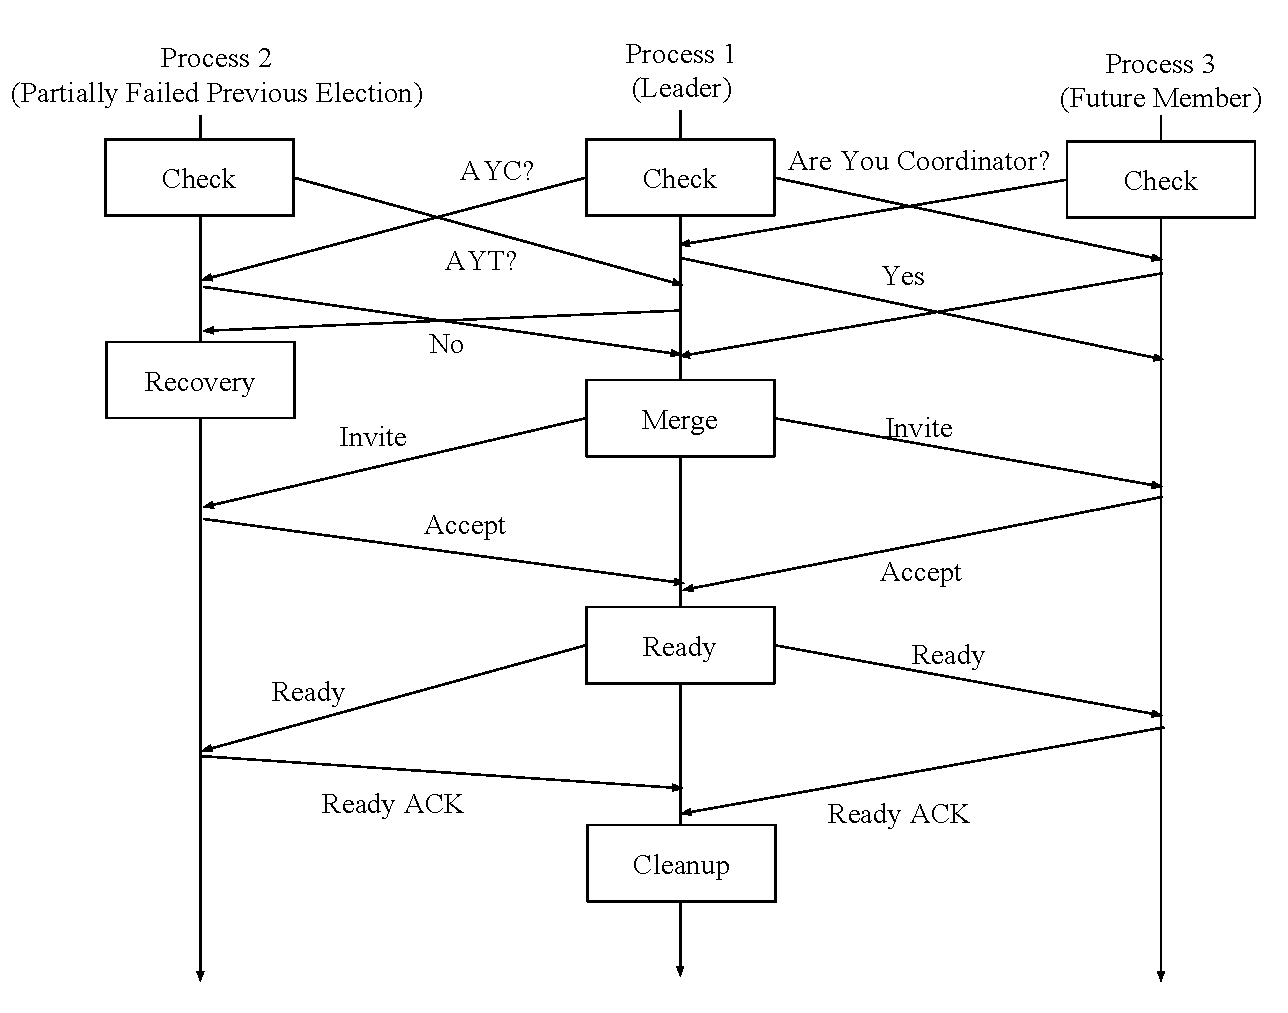
\includegraphics[width=\linewidth]{ElectionMessages}
\caption[Diagram of message exchanges for an election.]{Diagram of message exchanges for an election. Process 2 almost completed the previous election and considers itself a part of process 1's group, but process 1 does not. Process 3 does not consider itself a part of process 1's group before the election begins. Both process 2 and process 3 need to successfully exchange the same number of messages to successfully complete the election.}
\label{fig:electionmessages}
\end{figure}

% Stage 1: AYC / AYT
% Show that maint. takes so many messages
% Show that leader discovery for election takes so many messages
% Show that a process in M but not L needs to many messages to do the above, which is equal.
A process can update $L_i$ with leaked information.
To ensure the memorylessness property, we are particularly interested in the situation where a process receives the ready message, but the acknowledgment is lost, meaning the process is not included in the $L_i$ set.
We wish to ensure that the process can determine its own exclusion in $L_i$ so it can behave as though it is not in $M_i$.
To do this, we attach an additional field to the \ac{AYC} message to indicate if the coordinator $i$ considers the receiving process $j$ a part of the $L_i$ set.
The receiving process can infer it is not part of $L_i$ and it should behave accordingly.

Likewise, for the coordinator, an \ac{AYT} message leaks that the sending process is a part of the $M_i$ set if it is not in $L_i$.
Since the behavior of the process in $M_i$ is defined to behave as though it was not in $L_i$, the coordinator should do the same.
This should be the case even if the process sending \ac{AYT} has already responded negatively to an \ac{AYC} from $i$.
For the purpose of memorylessness, $i$ should consider $j$ to have responded in the affirmative.

% Stage 2:
% Show that the probability of an invite working is the probability of delivering an invite
% + all the lower priority invites not arriving
% Show that at this point M/L inclusion doesn't matter any more.
Processes determine which invitation to accept based on the exchange of the \ac{AYC} messages.
Processes always seek to reach the ``lowest energy state'': they wish to be in a group led by the coordinator with the highest priority.
Processes will submit AYC messages to higher priority processes that are not its coordinator, even if they are in a group.
As a result, the processes will always seek highest priority, regardless of their current group.
More importantly, this releases the process from obligations on its next state from the state of other processes in the system.
A process will only accept a received invitation if it has determined the sending process is the highest priority process.

% Stage 3:
% Show that ready only depends on the sucessful delivery of ready
% & Ready ack.

In Figure \ref{fig:electionmessages}, we diagram the sequence of message exchanges and function calls for two possible states for a process not in the leader's group.
In the first state, the process nearly completed an election the previous round, but the ready acknowledgement message was not delivered in time, resulting in the process being in the $M_i$ set.
In the second state, the process is not in the leader's group.
Both cases require the same number of messages to be delivered for the process to be considered a part of the group.

Therefore, regardless of the hidden state of the system, the highest priority process' observations will produce a Markov chain.
The probability of transitioning to the next state is not influenced by the interactions of the other processes: it only depends on the combinations of outcomes based on the current observable state.

\begin{thm}
    The observations of the highest priority process are sufficient for producing a Markov chain from the underlying \ac{HMM}.
\end{thm}

\begin{proof}
\begin{case}
    The system has one other process ($n=1$).
\end{case}

If there is only one other process, the probability of observing a group of two processes given the current state is a direct observation.

\begin{case}
    The system has two other processes ($n=2$).
\end{case}

In this case, there are 3 possible states for each of the other processes to be in: grouped with the highest priority process, ungrouped, and grouped without the highest priority process.
When the other processes are grouped with the highest priority process, the probability of the other processes remaining in the group depends on the probability the current grouping is maintained.
In the second scenario, where processes are ungrouped, the probability only depends on the probability they successfully contact the highest priority process.
The last scenario is identical to the second, as the processes will behave as though they are ungrouped when contacted by the highest priority process.

The only observation that can be made by the highest priority process is the inclusion or exclusion of the other processes in their group.
The probability of the processes excluded in the group joining the group is independent of their current state.
Let $X_G$ be the set of states for the \ac{HMM} where the other processes are excluded from $P_0$'s group, and in their own group led by $P_1$.
$X_U$ is the set of states where the processes are excluded from $P_0$'s group and are themselves ungrouped.
By the nature of the algorithm: 

\begin{equation}
\Pr(O(D_0, X_{k+1}) | X_k \in X_G) = \Pr(O(D_0, X_{k+1}) | X_k \in X_U).
\label{eq:sameprob}
\end{equation}

As a result, the ungrouped and grouped sub-cases have the same probability of resulting in a particular $Y_{k+1}$.
Furthermore, based on the observations of the ungrouped process:

\begin{equation}
O(D_0, x_i) = O(D_0, x_j), \forall x_i \in X_G, \forall x_j \in X_U.
\end{equation}

The equation indicates every observation of a state in $X_G$ and $X_U$ looks identical to $P_0$.
With this restriction:

\begin{equation}
\Pr(Y_{k+1} | Y_{k}) = \sum_{\{X_{k+1} | O(X_{k+1}) = Y_{k+1}\}} \Pr(X_{k+1} | X_{k}), \forall X_k \in \{X_k | X_k \in X_U \cup X_G\}.
\end{equation}

Where $X_U \cup X_G$ is the complete set of states for processes not in $P_0$'s group.

\begin{case}
    The system has a number of other processes ($n > 2$).
\end{case}

Since the interactions of the other processes do not affect the probability of joining $P_0$'s group, the previous case directly extends to this case.

\end{proof}

\subsection{Model Construction}

Based on the state determination and memorylessness arguments presented, the highest priority process operates independent of the state of the other processes in the system.
The structure of the algorithm prevents any process from being locked out of participating in a round of execution based on the outcome of the previous round.
Therefore, for every observation of the system state the highest priority process makes, the next round of execution for all the other processes favors the high priority process, ensuring that its observation corresponds directly with the system state.

The states of the Markov chain are the cardinality of the highest priority process' group.
In each round, the behavior is described by two components: maintaining a group and inviting other processes into the group.
The coordinator will exchange an ``Are You Coordinator'' message and the peer will respond to verify it is still available.
To maintain a group of $m$ other processes, the probability is defined as a random variable with the following \ac{pdf}:

\begin{equation}
 \Pr_{M}(Y=k; m) =
   \begin{cases}
    \binom{m}{k} p^{2k}(1-p^2)^{m-k}, & \text{if } 0 \leq k \leq m \\
    0,                                & \text{otherwise} \\
  \end{cases}
\end{equation}%
where $k$ is the number of processes remaining in a group selected from $m$ processes.
A process will leave a group if, from the considered process' perspective, they do not respond to an ``Are You Coordinator'' message.

To invite other processes to the group, the two processes ultimately exchange up to 8 messages.
In a round, a single process can invite many other processes to its group.
From a selection of $n$ other coordinators, the probability distribution for joining a new group with $k$ of the $n$ processes is:

\begin{equation}
    \Pr_{I}(Y=k; n) =
    \begin{cases}
        \binom{n}{k} p^{8k}(1-p^8)^{n-k}, & \text{if } 0 \leq k \leq n \\
        0,                                & \text{otherwise.} \\
    \end{cases}
\end{equation}

In the profile chain, in a state $s$ that describes the number of processes in a group, the probability of transitioning from $s$ to $s'$ with $n$ total processes (including the considered process) is:

\begin{align} \Pr_{T}(Z=s'; n; s) = \sum_{i=0}^{s-1} &\Pr_{M}(X=i; s-1) *
\nonumber \\ &\Pr_{I}(X=s'-i; n-s-1).\end{align}

From this distribution, a set of transition probabilities can be calculated for a given probability of delivery $p$ and number of processes $n$.
This set of transition probabilities forms a profile Markov chain $P$, which can be evaluated for any number of processes $n$ and probability of delivery $p$.
The generated profile chain is ergodic when $0<p<1.0$. The profile chain is a stationary Markov chain.

\subsection{Model Validation}

%State that verification of the profile chain via statistical tests is important. State that if P and T are ergodic stochastic sources and can generate similar sequences if they have the same transition probabilities. State that statistical tests can identify if two chains are different at some significant level.

To assert the closed-form profile chain accurately represents the implementation of the algorithm, it must be validated.
Since $T$ and $P$ are ergodic, they can be checked for equivalence using a goodness-of-fit test.
If the goodness-of-fit test indicates the chains are equivalent, they will generate similar sequences and have similar properties when analyzed.
Therefore, generated $P$ chains can be used to analyze the behavior of the algorithm during live execution with changing conditions.

To verify the test chain $T$ is equivalent to the profile chain $P$, a $\chi^2$ goodness-of-fit test is employed.
The null-hypothesis of the test ($H_{0}$) asserts the profile chain $P$ is equivalent to the test chain $T$:

\begin{equation} H_{0}: T = P.\end{equation}

With an alternative hypothesis that the two chains are not equivalent:

\begin{equation} H_{1}: T \neq P.\end{equation}

The $\chi^2$ test measures the goodness-of-fit for a complete chain by combining the measurements of goodness of fit for the transitions away from each state.
Therefore, the goodness of fit test for the chain is a summation of tests for each state:\cite{MARKOV3}

\begin{equation} \chi^2 = \sum_{i}^{m} \sum_{j}^{m} = \frac{n_{i}(P_{ij}-T_{ij})^2}{P_{ij}} \end{equation}%
where $n_{i}$ is the number of times the state $i$ was observed in the input sequence used to construct the test chain $T$.
The summation is distributed as $\chi^2$ with $m(m-1)$ \ac{DF} if all entries in $P_{ij}$ are non-zero.
In this work, all transitions in the profile Markov chain $P$ are non-zero when $0<p<1.0$.
However, the probability of some transitions may be extremely small.
The $\chi^2$ value was compared to a \ac{CV} giving a measure of how likely it was $H_{0}$ could not be rejected.
This work selected an $\alpha = 0.05$ significance level to reject the hypothesis $T=P$.

If the hypothesis $H_{0}$ were to be rejected, it would indicate the test chain and profile chain differ significantly.
As a consequence of rejecting the hypothesis, the implementation would have behavior from the generated closed-form solution.

To verify the model, it was compared to runs of an implementation of the algorithm.
Test data was collected for systems with 3, 4, 5 and 6 processes.
Information was collected from sufficiently long runs of the system with a delivery probability between 0.05 and 0.95 tested at intervals of 0.05.
Table \ref{tab:chisummary} shows the measured error and p-value for the worst observed error for each number of processes.
Since the measured error is less than the critical value and the p-value is greater than 0.05, we cannot reject $H_0$. 
As a consequence, the profile chains ($P$) are representative of the behavior of the algorithm.

\begin{table*}[!t]
\centering
\caption{Summary of $\chi^2$ tests performed.}
\begin{tabular}{ c | c c c c c}
  \hline
  Processes & DF & CV & Worst Error & $\Pr(WorstError)$ &  p-value \\ \hline
  3 & 6 & 12.6 & 8.90 & 0.80 & 0.18 \\
  4 & 12 & 21.0 & 14.55 & 0.75 & 0.27 \\
  5 & 20 & 31.4 & 23.47 & 0.65 & 0.27 \\
  6 & 30 & 43.8 & 32.69 & 0.85 & 0.34 \\
\end{tabular}

\label{tab:chisummary}
\end{table*}

\subsection{Profile Chain Analysis}

Resources can only be managed effectively when multiple \ac{DGI} coordinate together to manage those resources.
Without another DGI to coordinate with, the DGI has a limited range of options to manage power generation, storage, and loads.
Therefore, the amount of time the DGI will spend coordinating with another process is of particular interest.
\cite{CRITIS2012} defines an \ac{IGT} metric to measure the amount of time a DGI process spends coordinating with at least one other process.
In this work, we define \ac{IGT} based on the steady state of the profile chain.
Let $\pi=Steady(P)$ for some profile chain.
The \ac{IGT} is the sum of all states in $\pi$, save the first state where the process is alone:

\begin{equation} IGT = \sum_{i=2}^{m} \pi_i \end{equation}

The \ac{IGT} is a number between 0 and 1.
It represents the probability a random observation sees a group of at least two members.
The steady state distributions are presented as stacked bar graphs in Figures \ref{fig:ss-3process}, \ref{fig:ss-4process}, \ref{fig:ss-5process} and \ref{fig:ss-6process}.
Each complete bar in the graph indicates the \ac{IGT}.
Additionally, these figures contain the average group size (AGS) when the system has reached the steady-state plotted as a fraction of the total number of processes.
Let $P$ be the steady-state distribution vector for some number of processes, $n$, and a given probability of delivery rate:

\begin{equation} y = \frac{\sum_{i=1}^{n} P_{i}*i}{n} \label{eq:ss-means} \end{equation}

where $y$ is the plotted \ac{AGS} as a fraction.

The components of each bar represent the probability the system is in a specific state for a random observation of the system.
The height of the component represents the relative probability of observing that state when in a group.

\begin{figure}
    \centering
    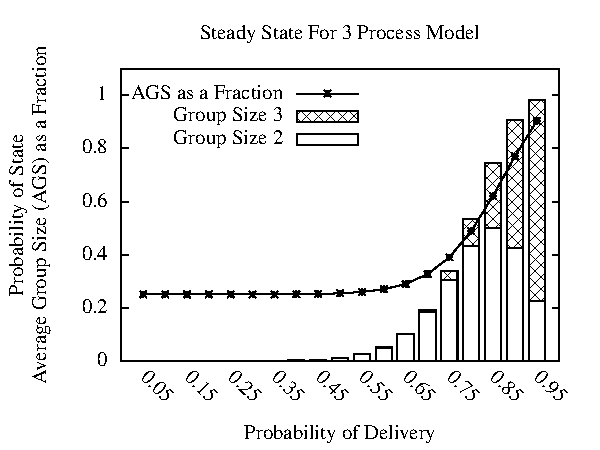
\includegraphics[width=0.6\linewidth]{ss-3process.pdf}
    \caption{Steady state distribution for 3 processes as well as the \ac{AGS} as a fraction of total processes.}
    \label{fig:ss-3process}
\end{figure}

\begin{figure}
    \centering
    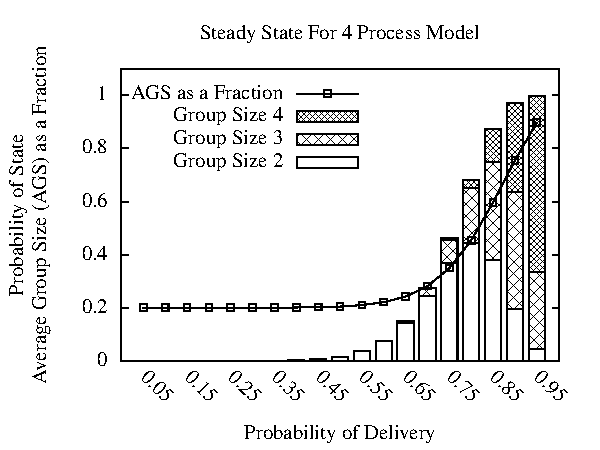
\includegraphics[width=0.6\linewidth]{ss-4process.pdf}
    \caption{Steady state distribution for 4 processes as well as the \ac{AGS} as a fraction of total processes.}
    \label{fig:ss-4process}
\end{figure}

\begin{figure}
    \centering
    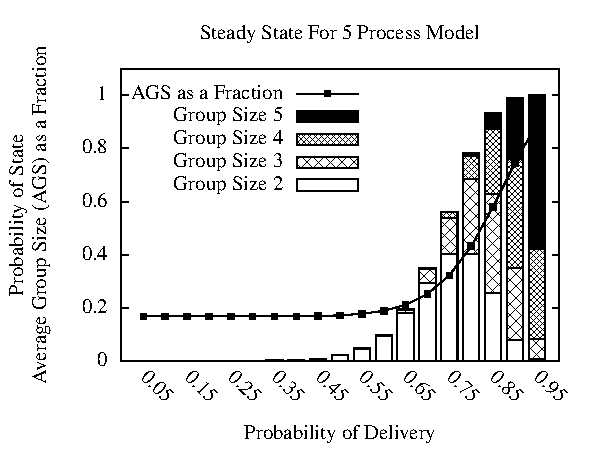
\includegraphics[width=0.6\linewidth]{ss-5process.pdf}
    \caption{Steady state distribution for 5 processes as well as the \ac{AGS} as a fraction of total processes.}
    \label{fig:ss-5process}
\end{figure}

\begin{figure}
    \centering
    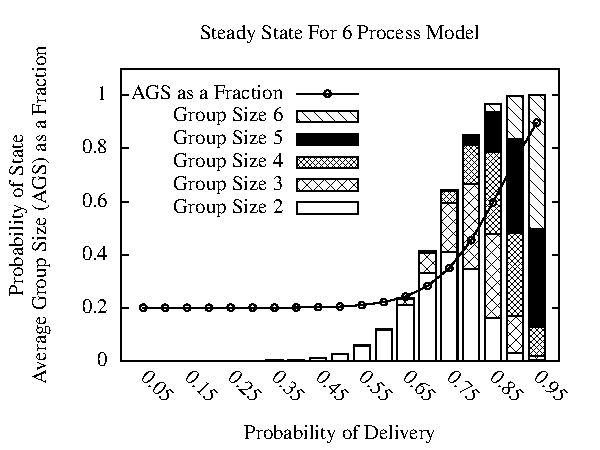
\includegraphics[width=0.6\linewidth]{ss-6process.pdf}
    \caption{Steady state distribution for 6 processes as well as the \ac{AGS} as a fraction of total processes.}
    \label{fig:ss-6process}
\end{figure}

The profile chain can be used to ensure the \ac{FREEDM} smart-grid is able to continue operating despite network issues.
The profile chain can be combined with different message-sending strategies to maintain service.
For example, the DGI can change its behavior to ensure operation continues normally despite connectivity issues.
By selecting different strategies depending on the message delivery probability, the DGI can offer high performance in good network conditions and an acceptable level of service during faults.
The profile chain can be extended to an arbitrary number of processes as shown in Figure \ref{fig:ss-means}.
In the figure, the steady-state of the system is used to compute a weighted average of the group size.
To compare the produced steady states, the weighted average is plotted as a percentage of all processes in the system.
Values in Figure \ref{fig:ss-means} are plotted using Equation \ref{eq:ss-means}.
Therefore, Figure \ref{fig:ss-means} shows the average percentage of total processes that will be in the group in a steady-state system.

\begin{figure}
    \centering
    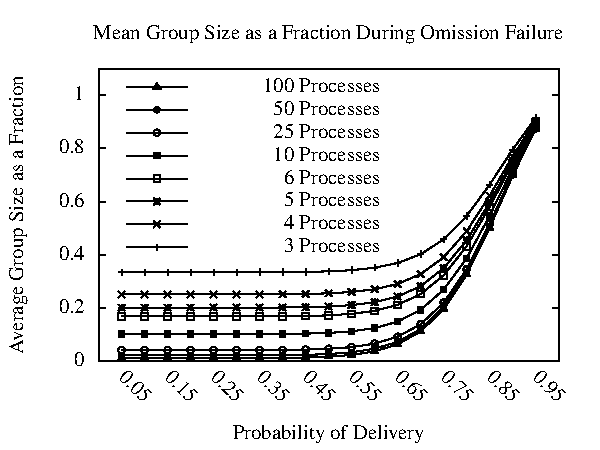
\includegraphics[width=0.6\linewidth]{ss-means.pdf}
    \caption{Average group size as a percentage of all processes in the system for larger systems.}
    \label{fig:ss-means}
\end{figure}


% For a lower priority process, the probability that an invite will work depends on the probability that that process is
% Not already in a higher priority group IE, it depends on the outcome of the last election & staying in a group this time
% For the highest priority process, it doesn't matter what the outcome of the last election was, it can merge that process into its group.
% So we can demonstrate 2 things: First, the probability of inviting a process from a lower priority process would violate the memorylessness property
% And secondly, the state of the other process being in the group is MSDND secure
% A result is secure until it is revealed and then when the process changes variables it is secure again.
%TODO...

% Set of worlds may need to be defined over a round of execution? Keep space smaller, fixes belief revision.
% You can show two worlds, one where the process is group and the other where its ungrouped have different outcomes
% for a third process.

% You can show that the there is no way for the process to know that, the state is MSDND secure.
% Lastly, we need to show there is no way of making it independent
% There's several different versions for this:
% It may be sufficent to show that it can only be memoryless for the leader, because only the highest priority
% can know that the invites will work, every other process depends on the state of the highest priority process
% which is not memoryless. No matter how it is defined, allowing a process with a higher priority to determine
% The state prevents a lower priority one from doing so.

% Really, the arguement is, if the state affects you can you can't determine it, you can't construct a model.
% Maybe as a corrollary?
% Well, in this case, the highest priority process is not affected by the state it doesn't know.
% Can I prove that if the markov chain is first order, some other process must always be affected by the hidden state?

%\section{Independent Algorithm}

%Algorithm X presents a leader election algorithm that fulfills the requirements for any process to model the algorithm.

% Interesting... can I prove that if any process depends on a previous state, no other process can be memoryless?

% Send an invite to each lower priority process. (Each receives n invites)
% Each process collects all the invites and selects the highest priority
% Send response to highest priority.
% Process sends ready to recipients
% recips send ready ack

% probability of success = probability higher priority's invites don't arrive.
% * the probability the response makes it
% * the probability the ready makes it
% * the probability the ready ack makes it


